\documentclass[12pt]{article}
 
\usepackage[margin=1in]{geometry} 
\usepackage{amsmath,amsthm,amssymb}
\usepackage{graphicx} 
\begin{document}
 
\title{Artficial Intelligence} 
\author{Mark Anderson\\ 
Homework 2} 
 
\maketitle
 
 
\paragraph{Missionaries and Cannibals}
\begin{enumerate}

  \item Precisely formulate the problem by:\par
  \begin{enumerate}
    \item Define a state by giving the minimal set of information needed to uniquely identify it.\par
      A state will be able to be identified by the following: \par
      \begin{itemize}
        \item Which side of the river you (the boat) are on (Right / Left)
        \item Number of cannibals present
        \item Number of missionaries present
      \end{itemize}
    \item Specifying the initial state\par
    The initial state will be on the Left side of the river with 3 Missionaries and 3 Cannibals

    \item Defining a function ACTIONS(s) for an arbitrary state s which returns the set of actions that can be executed in state s.
    The actions available to an arbitrary state s are:
      \begin{itemize}
        \item MOVE(numCannibals, numMissionaries): Crosses the river with the specified number of cannibals/missionaries, because there are only 2 sides possible there is no need to specify direction.  May result in a dead state based on this action, and the maximum number occupants may not exceed 2.
      \end{itemize}

    \item Defining a transition model by specifying a function RESULT(s,a) which returns the state that results from executing action a in state s.
    Transition Model:
      \begin{itemize}
        \item RESULT(s, MOVE(numCannibals, numMissionaries)): Switches the agent to the opposite state along with the modified number of cannibals/missionaries ferried.  This costs one point. 
      \end{itemize}
    \item Defining a test to determine whether a given state is a goal state.\par
    If the agent is on the Right side of the river with 3 missionaries and 3 cannibals you are in the goal state.

    \item Defining the step cost (which also gives us the past cost as that's merely the sum of all the step costs associated with a path).\par
    Every instance of MOVE() called costs one step.
  \end{enumerate}

  \item Professional render a diagram of the complete state space employing appropriate software such as Microsoft Visio or the free open-source software Dia.\par
  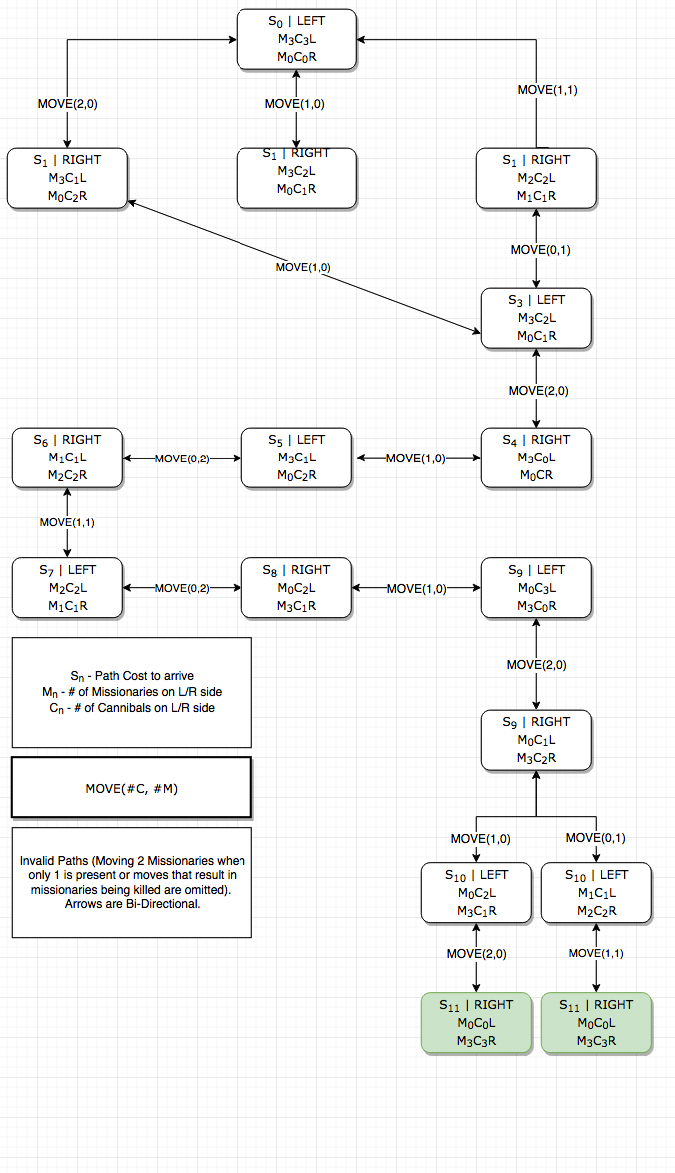
\includegraphics[width=\textwidth]{StateGraph.png}

  \item Find and report a path in the state space from the initial state to a goal state (i.e., a solution).\par
  \begin{enumerate}
    \item MOVE(1,1) -- Cross with 1 Missionary and 1 Cannibal 
    \item MOVE(0,1) -- Cross with 1 Missionary
    \item MOVE(2,0) -- Cross with 2 Cannibals
    \item MOVE(1,0) -- Cross with 1 Cannibal
    \item MOVE(0,2) -- Cross with 2 Missionaries
    \item MOVE(1,1) -- Cross with 1 Missionary and 1 Cannibal
    \item MOVE(0,2) -- Cross with 2 Missionaries
    \item MOVE(1,0) -- Cross with 1 Cannibal
    \item MOVE(2,0) -- Cross with 2 Cannibals
    \item MOVE(1,0) -- Cross with 1 Cannibal
    \item MOVE(2,0) -- Cross with 2 Cannibals
  \end{enumerate}
\end{enumerate}



\end{document}
